%==============================================================
%  EE201 -- Circuit Theory I
%  Lecture 4 : The Capacitor
%  M. Mert Ankaralı, METU EEE
%
%  Compile:  ./build.sh      (or: pdflatex EE201_Lecture_4.tex, twice)
%==============================================================
\documentclass[11pt,a4paper]{article}

%-------------------- packages --------------------------------
\usepackage[T1]{fontenc}
\usepackage[utf8]{inputenc}
\usepackage[english]{babel}
\usepackage{lmodern}
\usepackage[margin=2.3cm,top=2.0cm,bottom=1.9cm,headheight=14pt,headsep=9pt]{geometry}
\usepackage{amsmath,amssymb}
\usepackage{array,booktabs,tabularx}
\usepackage{enumitem}
\usepackage[table]{xcolor}
\usepackage{fancyhdr}
\usepackage{titlesec}
\usepackage{graphicx}
\usepackage[most]{tcolorbox}
\usepackage{tikz}
\usepackage[american,siunitx]{circuitikz}
\usetikzlibrary{arrows.meta,positioning,calc,decorations.pathmorphing,decorations.pathreplacing,decorations.markings,patterns,shapes.geometric}
\usepackage[colorlinks=true,allcolors=metured,breaklinks=true]{hyperref}

%-------------------- colour system ---------------------------
% One colour per physical quantity, used identically in the slides.
\definecolor{metured}{RGB}{155,27,48}    % headings, structure
\definecolor{metugray}{RGB}{88,89,91}
\definecolor{ccur}{RGB}{0,102,170}       % CURRENT  -- blue
\definecolor{cvolt}{RGB}{214,120,0}      % VOLTAGE  -- orange
\definecolor{cpow}{RGB}{23,128,74}       % POWER / ENERGY -- green
\definecolor{ccharge}{RGB}{124,60,160}   % CHARGE   -- purple
\definecolor{boxgray}{RGB}{245,245,245}

\newcommand{\Icol}[1]{\textcolor{ccur}{#1}}
\newcommand{\Vcol}[1]{\textcolor{cvolt}{#1}}
\newcommand{\Pcol}[1]{\textcolor{cpow}{#1}}
\newcommand{\Qcol}[1]{\textcolor{ccharge}{#1}}

%-------------------- units (no siunitx dependency) -----------
\newcommand{\uni}[1]{\,\mathrm{#1}}
\newcommand{\A}{\uni{A}}   \newcommand{\V}{\uni{V}}
\newcommand{\W}{\uni{W}}   \newcommand{\J}{\uni{J}}
\newcommand{\Cb}{\uni{C}}  \newcommand{\s}{\uni{s}}

%-------------------- layout ----------------------------------
\pagestyle{fancy}
\fancyhf{}
\lhead{\small\textcolor{metugray}{EE201 -- Circuit Theory I}}
\rhead{\small\textcolor{metugray}{Lecture 4: The Capacitor}}
\cfoot{\small\thepage}
\renewcommand{\headrulewidth}{0.4pt}

\titleformat{\section}{\large\bfseries\color{metured}}{\thesection.}{0.6em}{}
\titleformat{\subsection}{\normalsize\bfseries\color{metugray}}{\thesubsection.}{0.6em}{}
\titlespacing*{\section}{0pt}{1.4ex plus .3ex}{0.7ex}
\titlespacing*{\subsection}{0pt}{1.1ex plus .2ex}{0.5ex}

\setlist[itemize]{itemsep=2pt,topsep=3pt,parsep=0pt,leftmargin=1.5em}
\setlist[enumerate]{itemsep=2pt,topsep=3pt,parsep=0pt,leftmargin=1.7em}
\setlength{\parindent}{0pt}
\setlength{\parskip}{0.7ex plus .1ex}
\raggedbottom
\widowpenalty=10000
\clubpenalty=10000
\brokenpenalty=10000

%-------------------- boxes -----------------------------------
\newtcolorbox{definitionbox}[1]{enhanced,
  colback=metured!4, colframe=metured, boxrule=0.9pt,
  fonttitle=\bfseries, title={#1}, arc=2pt,
  left=7pt,right=7pt,top=5pt,bottom=5pt, before skip=7pt, after skip=7pt}

\newtcolorbox{ideabox}[1][Key idea]{enhanced,
  colback=ccur!5, colframe=ccur, boxrule=0.9pt,
  fonttitle=\bfseries, title={#1}, arc=2pt,
  left=7pt,right=7pt,top=5pt,bottom=5pt, before skip=7pt, after skip=7pt}

\newtcolorbox{examplebox}[1][Example]{enhanced,
  colback=cpow!4, colframe=cpow, boxrule=0.9pt,
  fonttitle=\bfseries, title={#1}, arc=2pt,
  left=7pt,right=7pt,top=5pt,bottom=5pt, before skip=7pt, after skip=7pt}

\newtcolorbox{cautionbox}[1][Careful]{enhanced,
  colback=cvolt!6, colframe=cvolt, boxrule=0.9pt,
  fonttitle=\bfseries, title={#1}, arc=2pt,
  left=7pt,right=7pt,top=5pt,bottom=5pt, before skip=7pt, after skip=7pt}

%-------------------- circuitikz defaults ---------------------
\ctikzset{bipoles/length=0.9cm, color=black,
          label/align=straight,
          bipoles/vsourceam/height=0.85, bipoles/vsourceam/width=0.85}
\tikzset{
  curarr/.style={-{Stealth[length=2.6mm]}, ccur, very thick},
  volarr/.style={-{Stealth[length=2.6mm]}, cvolt, very thick},
  blk/.style={draw=metugray, fill=boxgray, rounded corners=2pt,
              minimum height=1.25cm, text width=2.9cm, align=center, font=\small},
  flowarr/.style={-{Stealth[length=3mm]}, metured, very thick},
}

%==============================================================

%-------------------- extra macros for this lecture -----------
\newcommand{\ohm}{\,\Omega}
\newcommand{\kohm}{\,\mathrm{k}\Omega}
\newcommand{\Req}{R_{\mathrm{eq}}}
%  v--i axes:  #1 half-width, #2 half-height, #3 caption under the frame
\newcommand{\viaxes}[3]{%
  \draw[vax] (-#1,0) -- (#1,0) node[right=1pt, font=\scriptsize, text=cvolt] {$v$};
  \draw[vax] (0,-#2) -- (0,#2) node[above=1pt, font=\scriptsize, text=ccur] {$i$};
  \node[ttl] at (0,-#2-0.68) {#3};}
%  q--v axes: voltage across, charge stored
\newcommand{\qvaxes}[3]{%
  \draw[vax] (-#1,0) -- (#1,0) node[right=1pt, font=\scriptsize, text=cvolt] {$v$};
  \draw[vax] (0,-#2) -- (0,#2) node[above=1pt, font=\scriptsize, text=ccharge] {$q$};
  \node[ttl] at (0,-#2-0.68) {#3};}
%  t axes for waveforms
\newcommand{\taxes}[4]{%
  \draw[vax] (-0.15,0) -- (#1,0) node[right=1pt, font=\scriptsize] {$t$};
  \draw[vax] (0,-#2) -- (0,#3) node[above=1pt, font=\scriptsize] {#4};}
\tikzset{
  gnode/.style={circle, fill=metured, inner sep=0pt, minimum size=4.2pt},
  glab/.style={font=\footnotesize, text=metured},
  barr/.style={-{Stealth[length=2.2mm]}, metugray, thick},
  surf/.style={draw=cpow, very thick, dashed, rounded corners=6pt},
  vax/.style={-{Stealth[length=2mm]}, gray!70},
  crv/.style={metured, very thick},
  ttl/.style={font=\scriptsize\bfseries, text=metugray},
  gbr/.style={metugray, thick, postaction={decorate, decoration={markings,
      mark=at position 0.58 with {\arrow{Stealth[length=2.4mm]}}}}},
  pol/.style={font=\small, text=cvolt},
  iar/.style={-{Stealth[length=2.4mm]}, ccur, very thick},
}

%==============================================================
\begin{document}

%-------------------- title block -----------------------------
\begin{center}
\begin{tcolorbox}[enhanced, colback=metured!5, colframe=metured, boxrule=1pt,
                  arc=3pt, left=10pt,right=10pt,top=7pt,bottom=7pt, width=\textwidth]
\begin{center}
  {\small\scshape Middle East Technical University}\\[2pt]
  {\small\scshape Department of Electrical and Electronics Engineering}\\[7pt]
  {\Large\bfseries\color{metured} EE201 -- Circuit Theory I}\\[4pt]
  {\large\bfseries Lecture 4: The Capacitor}\\[6pt]
  {\small M. Mert Ankaralı}
\end{center}
\end{tcolorbox}
\end{center}
\vspace{-0.5em}

\begin{center}
\small
\begin{tabular}{@{}l l@{}}
\toprule
\multicolumn{2}{@{}l}{\textbf{Colour code used in these notes and in the slides}}\\
\midrule
\Qcol{$\blacksquare$}~charge $q$ & \Icol{$\blacksquare$}~current $i$ \quad
\Vcol{$\blacksquare$}~voltage $v$ \quad \Pcol{$\blacksquare$}~power $p$, energy $w$\\
\bottomrule
\end{tabular}
\end{center}

%==============================================================
\section{An element that stores energy}

Every element so far --- sources, diodes, the LTI resistor --- has been a \emph{resistor}
in the sense of Lecture~3: its characteristic is a curve in the $\Vcol{v}$--$\Icol{i}$
plane, so the present current is fixed by the present voltage and nothing else. Look at
what that does to energy. In a resistor $\Pcol{p} = R\Icol{i}^2 \ge 0$ at every instant:
the element \textbf{dissipates} the energy it is given, turning it into heat and letting
it go. It flows one way only, and none of it ever comes back.

Today's element dissipates nothing. Energy goes in, \emph{stays} in, and comes back out
later when the circuit asks for it --- all of it. A capacitor is an \textbf{ideal
energy-storage element}, and that is also why it remembers: what it does now depends on
everything that has been put into it.

\begin{center}
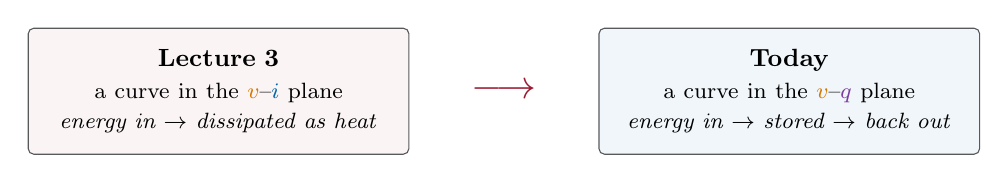
\begin{tikzpicture}[node distance=0.9cm]
  \node[blk, text width=4.6cm, minimum height=1.6cm, fill=metured!5] (a)
       {\textbf{Lecture 3}\\[2pt]\footnotesize a curve in the
        $\Vcol{v}$--$\Icol{i}$ plane\\ \footnotesize \emph{energy in $\to$ dissipated as heat}};
  \node[blk, text width=4.6cm, minimum height=1.6cm, right=2.4cm of a, fill=ccur!6] (b)
       {\textbf{Today}\\[2pt]\footnotesize a curve in the
        $\Vcol{v}$--$\Qcol{q}$ plane\\ \footnotesize \emph{energy in $\to$ stored $\to$ back out}};
  \node[font=\Large, text=metured] at ($(a)!0.5!(b)$) {$\longrightarrow$};
\end{tikzpicture}
\end{center}

\subsection{Why energy is the bigger idea}

Charge is the natural bookkeeping variable inside an electrical circuit, and the next few
pages are written in terms of it. But charge only means something electrically. Energy
means the same thing everywhere --- and an ideal energy-storage element is a shape that every
physical domain has:

\begin{center}
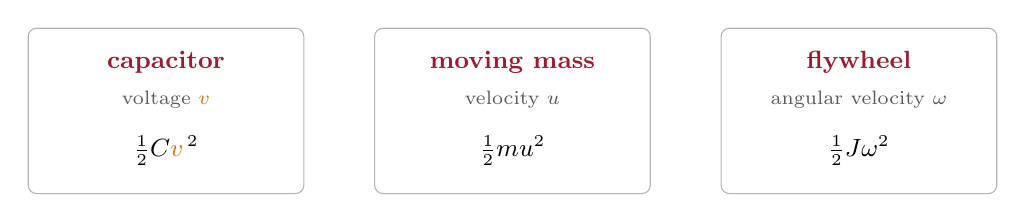
\begin{tikzpicture}[x=1cm,y=1cm]
  \foreach \dx/\ttl/\sub/\expr in {0/{capacitor}/{voltage $\Vcol{v}$}/{$\tfrac12 C\Vcol{v}^{\,2}$},
                              4.4/{moving mass}/{velocity $u$}/{$\tfrac12 m u^2$},
                              8.8/{flywheel}/{angular velocity $\omega$}/{$\tfrac12 J\omega^2$}}{
    \begin{scope}[xshift=\dx cm]
      \draw[metugray!45, rounded corners=3pt] (-1.75,-1.05) rectangle (1.75,1.05);
      \node[font=\small\bfseries, text=metured] at (0,0.62) {\ttl};
      \node[font=\scriptsize, text=metugray] at (0,0.14) {\sub};
      \node[font=\small] at (0,-0.5) {\expr};
    \end{scope}}
\end{tikzpicture}
\end{center}

Each one takes energy in, holds it, and gives it back --- and in each the stored energy is
half a constant times the square of one variable. The resistor's mechanical counterpart is
\emph{viscous friction}: it too takes energy in, and there the resemblance stops.
Lecture~1 lined the domains up variable by variable; this is the same table read one level
higher, in the one quantity they all share.

%==============================================================
\section{The capacitor: a curve in a different plane}

Some elements store charge. For those, the useful pair of variables is not
$(\Vcol{v},\Icol{i})$ but $(\Vcol{v},\Qcol{q})$, where $\Qcol{q(t)}$ is the charge that has
entered the $+$ terminal:
\[
  \Qcol{q(t)} \;=\; \Qcol{q(t_0)} + \int_{t_0}^{t}\!\Icol{i(\tau)}\,d\tau
  \qquad\Longleftrightarrow\qquad
  \Icol{i} = \frac{d\Qcol{q}}{dt} \quad\text{(Lecture 1)} .
\]

\begin{definitionbox}{Capacitor}
A two-terminal element is a \textbf{capacitor} if, at every instant, its
$(\Vcol{v},\Qcol{q})$ pairs lie on a curve in the $\Vcol{v}$--$\Qcol{q}$ plane.
\end{definitionbox}

\begin{center}
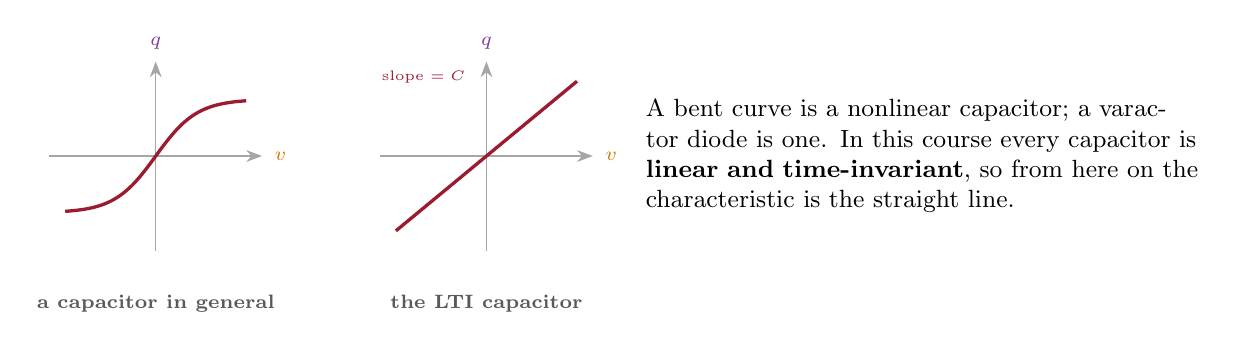
\begin{tikzpicture}[x=1cm,y=1cm]
\begin{scope}
  \qvaxes{1.35}{1.2}{a capacitor in general}
  \draw[crv, domain=-1.15:1.15, samples=140, smooth] plot (\x, {0.72*tanh(1.9*\x)});
\end{scope}
\begin{scope}[xshift=4.2cm]
  \qvaxes{1.35}{1.2}{the LTI capacitor}
  \draw[crv] (-1.15,-0.95) -- (1.15,0.95);
  \node[font=\tiny, text=metured] at (-0.80,1.00) {slope $=C$};
\end{scope}
\node[font=\small, anchor=west, text width=7.2cm] at (6.1,0)
  {A bent curve is a nonlinear capacitor; a varactor diode is one. In this course every
   capacitor is \textbf{linear and time-invariant}, so from here on the characteristic is
   the straight line.};
\end{tikzpicture}
\end{center}
\vspace{2pt}

Note what has \emph{not} happened. There is of course a relation between $\Vcol{v}$ and
$\Icol{i}$ --- we derive it two pages from here --- but it is not a relation between their
\emph{values at one instant}. For a capacitor there is no function $f$ or $g$ with
\[
  \Icol{i(t)} = f\bigl(\Vcol{v(t)}\bigr)
  \qquad\text{or}\qquad
  \Vcol{v(t)} = g\bigl(\Icol{i(t)}\bigr) .
\]
Fix the voltage at some value and the current is still free: it depends on how $\Vcol{v}$
is \emph{changing}, not on what it is. So a capacitor is not a resistor, and it has no
characteristic in the $\Vcol{v}$--$\Icol{i}$ plane at all.

\begin{center}
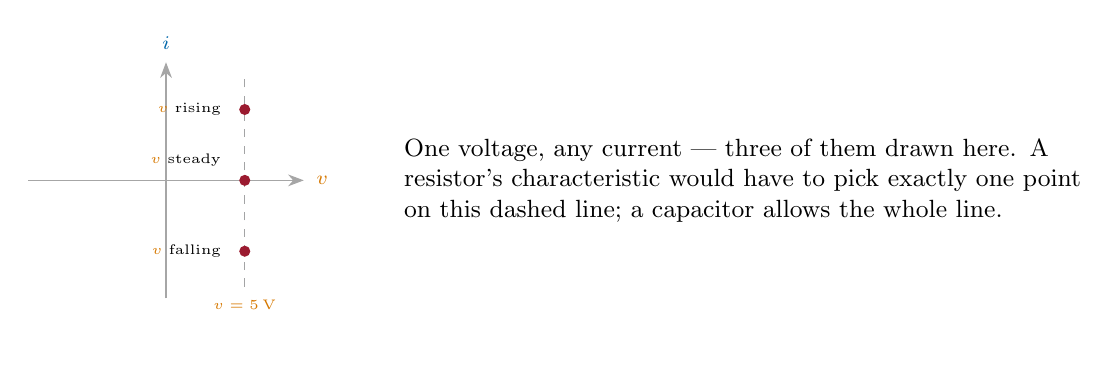
\begin{tikzpicture}[x=1cm,y=1cm]
  \viaxes{1.75}{1.5}{}
  \draw[metugray!55, dashed] (1.0,-1.35) -- (1.0,1.35);
  \node[font=\tiny, text=cvolt, below] at (1.0,-1.4) {$\Vcol{v} = 5\V$};
  \fill[metured] (1.0,0.9) circle (2.0pt);
  \fill[metured] (1.0,0) circle (2.0pt);
  \fill[metured] (1.0,-0.9) circle (2.0pt);
  \node[font=\tiny, anchor=east] at (0.82,0.9) {$\Vcol{v}$ rising};
  \node[font=\tiny, anchor=east] at (0.82,0.26) {$\Vcol{v}$ steady};
  \node[font=\tiny, anchor=east] at (0.82,-0.9) {$\Vcol{v}$ falling};
  \node[font=\small, anchor=west, text width=8.6cm] at (2.9,0)
    {One voltage, any current --- three of them drawn here. A resistor's characteristic
     would have to pick exactly one point on this dashed line; a capacitor allows the
     whole line.};
\end{tikzpicture}
\end{center}

%==============================================================
\section{Where the charge sits: the parallel-plate capacitor}

Two conducting plates of area $A$, a distance $d$ apart, with an insulator of permittivity
$\varepsilon$ between them. Push charge $+\Qcol{q}$ onto one plate and the same amount
leaves the other, so that plate carries $-\Qcol{q}$; the circuit outside never sees any
net charge appear or vanish.

\begin{center}
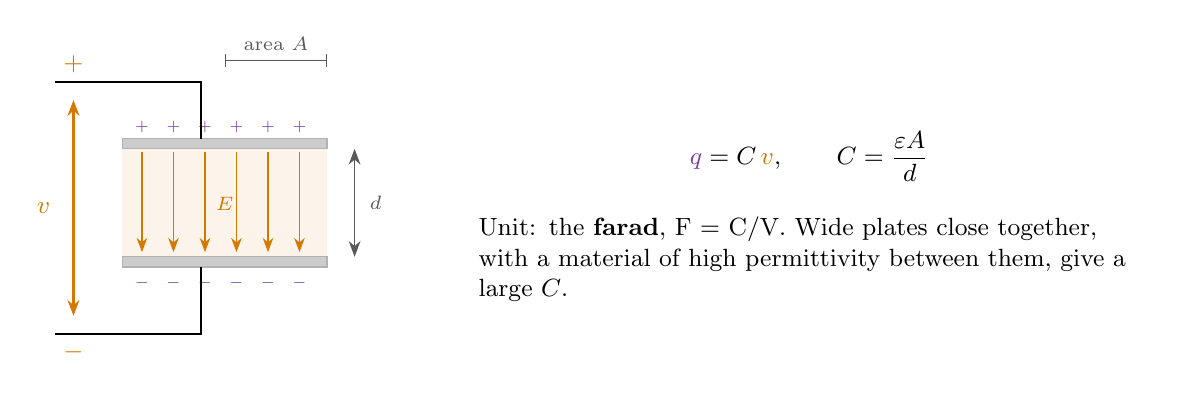
\begin{tikzpicture}[scale=1.0]
%---- the plates
\fill[gray!40] (0,0) rectangle (2.6,0.13);
\fill[gray!40] (0,1.5) rectangle (2.6,1.63);
\fill[cvolt!8] (0,0.13) rectangle (2.6,1.5);
\draw[gray!60] (0,0) rectangle (2.6,0.13);
\draw[gray!60] (0,1.5) rectangle (2.6,1.63);
\foreach \x in {0.25,0.65,1.05,1.45,1.85,2.25}{
  \draw[cvolt, -{Stealth[length=1.8mm]}] (\x,1.46) -- (\x,0.19);
  \node[font=\tiny, text=ccharge] at (\x,1.78) {$+$};
  \node[font=\tiny, text=ccharge] at (\x,-0.2) {$-$};}
\node[font=\scriptsize, text=cvolt] at (1.3,0.8) {$E$};
\draw[{Stealth[length=2mm]}-{Stealth[length=2mm]}, metugray]
      (2.95,0.13) -- (2.95,1.5);
\node[font=\scriptsize, text=metugray, right=2pt] at (2.95,0.82) {$d$};
\draw[metugray, |-|] (1.3,2.62) -- (2.6,2.62);
\node[font=\scriptsize, text=metugray, above] at (1.95,2.63) {area $A$};
\draw[thick] (1.0,1.63) -- (1.0,2.35) -- (-0.85,2.35);
\draw[thick] (1.0,0) -- (1.0,-0.85) -- (-0.85,-0.85);
\node[pol] at (-0.62,2.58) {$+$}; \node[pol] at (-0.62,-1.08) {$-$};
\draw[{Stealth[length=2mm]}-{Stealth[length=2mm]}, cvolt, very thick]
      (-0.62,-0.62) -- (-0.62,2.12);
\node[pol] at (-1.0,0.75) {$v$};
%---- the formula
\node[font=\small, anchor=west, text width=8.4cm] at (4.4,0.8)
  {\begin{center}
     $\displaystyle \Qcol{q} = C\,\Vcol{v}, \qquad C = \frac{\varepsilon A}{d}$
   \end{center}
   \vspace{4pt}
   Unit: the \textbf{farad}, F $=$ C/V. Wide plates close together, with a material of
   high permittivity between them, give a large $C$.};
\end{tikzpicture}
\end{center}
\vspace{2pt}

\begin{cautionbox}[One farad is enormous]
Plates of $1\uni{cm^2}$ separated by $0.1\uni{mm}$ of air give
\[
  C = \frac{\varepsilon_0 A}{d}
    = \frac{(8.85\times 10^{-12})(10^{-4})}{10^{-4}}
    \approx 8.9\uni{pF} .
\]
That is why practical values are quoted in pF, nF and $\mu$F, and why a $1\uni{F}$
supercapacitor has to roll an enormous area into a small can.
\end{cautionbox}

%==============================================================
\section{The LTI capacitor}

\begin{definitionbox}{LTI capacitor}
The $\Vcol{v}$--$\Qcol{q}$ characteristic is a fixed straight line through the origin,
$\Qcol{q} = C\,\Vcol{v}$ with $C$ constant. Differentiating and using
$\Icol{i} = d\Qcol{q}/dt$,
\[
  \boxed{\;\Icol{i} \;=\; C\,\frac{d\Vcol{v}}{dt}\;}
  \qquad\text{or, integrated,}\qquad
  \boxed{\;\Vcol{v(t)} = \Vcol{v(t_0)} + \frac{1}{C}\int_{t_0}^{t}\!\Icol{i(\tau)}\,d\tau\;}
\]
\end{definitionbox}

\begin{center}
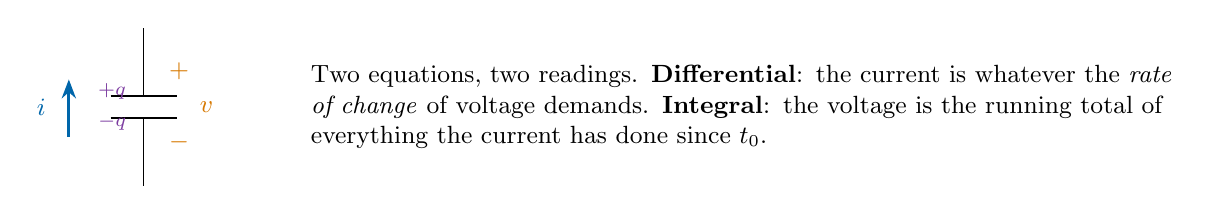
\begin{tikzpicture}[scale=1.0]
  \draw (0,0) to[C] (0,2.0);
  \node[pol] at (0.45,1.45) {$+$}; \node[pol] at (0.45,0.55) {$-$};
  \node[pol] at (0.8,1.0) {$v$};
  \draw[iar] (-0.95,0.62) -- (-0.95,1.35); \node[ccur, font=\small] at (-1.3,1.0) {$i$};
  \node[font=\scriptsize, text=ccharge] at (-0.4,1.2) {$+q$};
  \node[font=\scriptsize, text=ccharge] at (-0.4,0.8) {$-q$};
  \node[font=\small, anchor=west, text width=11.0cm] at (2.0,1.0)
    {Two equations, two readings. \textbf{Differential}: the current is whatever the
     \emph{rate of change} of voltage demands. \textbf{Integral}: the voltage is the
     running total of everything the current has done since $t_0$.};
\end{tikzpicture}
\end{center}
\vspace{2pt}

\begin{ideabox}[Four consequences, straight from the two boxes]
\begin{itemize}
  \item \textbf{At DC it is an open circuit.} $\Vcol{v}$ constant $\Rightarrow
        d\Vcol{v}/dt = 0 \Rightarrow \Icol{i} = 0$, whatever the voltage is.
  \item \textbf{Voltage cannot jump} --- not with a finite current. A step in $\Vcol{v}$
        would need $d\Vcol{v}/dt = \infty$.
  \item \textbf{It remembers.} $\Vcol{v(t)}$ depends on the whole history of $\Icol{i}$,
        not on its present value. A resistor knows only now; a capacitor knows everything
        that has happened to it.
  \item \textbf{It holds energy}, and the amount is $\Pcol{w} = \tfrac12 C\Vcol{v}^{\,2}$
        --- fixed by the present voltage alone. Section~\ref{sec:energy} shows why, and
        that every joule of it can be taken back out.
\end{itemize}
\end{ideabox}

%==============================================================
\section{Two examples that show the two readings}

\begin{examplebox}[Example 4.1 --- drive it with a constant current]
A current source pushes a constant $\Icol{I} = 1\uni{mA}$ into $C = 1\uni{\mu F}$, starting
from $\Vcol{v(0)} = 0$. The integral form gives
\[
  \Vcol{v(t)} = \frac{1}{C}\int_0^t \Icol{I}\,d\tau = \frac{\Icol{I}}{C}\,t
  = \frac{10^{-3}}{10^{-6}}\,t = 1000\,t \quad [\mathrm{V}] .
\]
A \textbf{ramp}: the voltage climbs at $1000\uni{V/s}$, reaching $5\V$ after $5\uni{ms}$.

\begin{center}
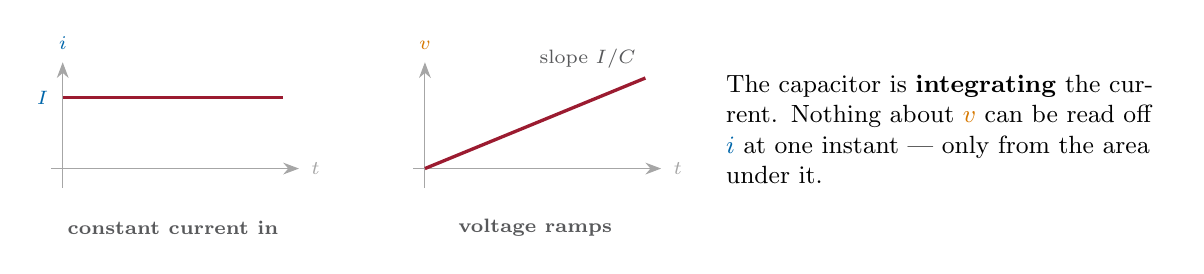
\begin{tikzpicture}[scale=1.0]
\begin{scope}
  \taxes{3.0}{0.25}{1.35}{\Icol{$i$}}
  \draw[crv] (0,0.9) -- (2.8,0.9);
  \node[font=\scriptsize, text=ccur, left] at (-0.06,0.9) {$I$};
  \node[ttl] at (1.4,-0.75) {constant current in};
\end{scope}
\begin{scope}[xshift=4.6cm]
  \taxes{3.0}{0.25}{1.35}{\Vcol{$v$}}
  \draw[crv] (0,0) -- (2.8,1.15);
  \node[font=\scriptsize, text=metugray, above left] at (2.8,1.15) {slope $I/C$};
  \node[ttl] at (1.4,-0.75) {voltage ramps};
\end{scope}
\node[font=\small, anchor=west, text width=5.6cm] at (8.3,0.5)
  {The capacitor is \textbf{integrating} the current. Nothing about $\Vcol{v}$ can be read
   off $\Icol{i}$ at one instant --- only from the area under it.};
\end{tikzpicture}
\end{center}
\vspace{-2pt}
In practice the ramp cannot go on for ever: the source will run out of voltage. Until it
does, this is exactly how a sawtooth generator works.
\end{examplebox}

\subsection{A first look at the impulse}
\label{sec:impulse}

The next example needs a signal we have not met. Start with an ordinary rectangular pulse
of height $h$ and width $1/h$, beginning at $t = 0$:

\begin{center}
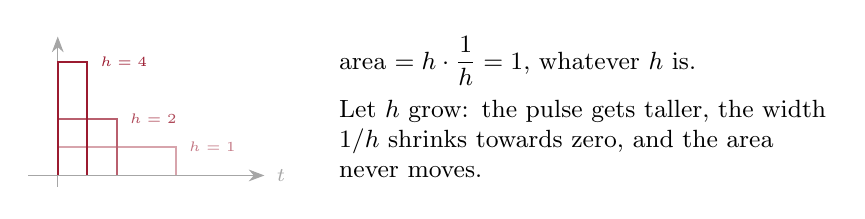
\begin{tikzpicture}[x=1.5cm, y=0.36cm]
  \draw[vax] (-0.25,0) -- (1.75,0) node[right=1pt, font=\scriptsize] {$t$};
  \draw[vax] (0,-0.4) -- (0,4.9);
  \draw[metured!40, thick] (0,0) -- (0,1) -- (1.0,1) -- (1.0,0);
  \node[font=\tiny, text=metured!60, right] at (1.03,1) {$h = 1$};
  \draw[metured!70, thick] (0,0) -- (0,2) -- (0.5,2) -- (0.5,0);
  \node[font=\tiny, text=metured!80, right] at (0.53,2) {$h = 2$};
  \draw[metured, thick] (0,0) -- (0,4) -- (0.25,4) -- (0.25,0);
  \node[font=\tiny, text=metured, right] at (0.28,4) {$h = 4$};
  \node[font=\small, anchor=west, text width=6.2cm] at (2.3,2.4)
    {area $= h \cdot \dfrac{1}{h} = 1$, whatever $h$ is.\\[4pt]
     Let $h$ grow: the pulse gets taller, the width $1/h$ shrinks towards zero, and the
     area never moves.};
\end{tikzpicture}
\end{center}

In the limit nothing is left that we could call a value --- the pulse is zero everywhere
except at $t = 0$, where it has run off to infinity --- but the \emph{area} is still
exactly $1$. That limit is the \textbf{unit impulse} $\delta(t)$.

\begin{definitionbox}{Unit impulse $\delta(t)$}
$\delta(t) = 0$ for every $t \neq 0$, and
\[
  \int_{a}^{b} \delta(\tau)\,d\tau = 1 \quad\text{for any } a < 0 < b .
\]
It is not a function in the ordinary sense; it is defined by the area it carries. Scaling
scales the area: $K\,\delta(t)$ has area $K$. We draw it as a vertical arrow, and the
number written beside the arrow is its \textbf{area}, never a height.
\end{definitionbox}

Two facts we will use straight away. First, a current impulse $K\,\delta(t)$ delivers
charge $K$ in zero time, since charge is the area under the current. Second, the impulse
is what you get by differentiating a step: if $\Vcol{v}$ jumps by $V$ at $t = 0$, then
$d\Vcol{v}/dt = V\,\delta(t)$ --- zero before, zero after, and area $V$ at the jump.

\begin{examplebox}[Example 4.2 --- drive it with a constant voltage]
Now hold $\Vcol{v} = V$ constant. Then $d\Vcol{v}/dt = 0$, so
\[
  \Icol{i} = C\,\frac{d\Vcol{v}}{dt} = 0 ,
  \qquad \Qcol{q} = C\,V \ \text{ sits on the plates and stays there.}
\]
The capacitor has become an \emph{open circuit}, and it stores $\Qcol{q} = CV$ while it
does so.
\vspace{4pt}

\textbf{But how did the voltage get there?} Compare two circuits, both driven by a source
that steps from $0$ to $V$ at $t = 0$.

\begin{center}
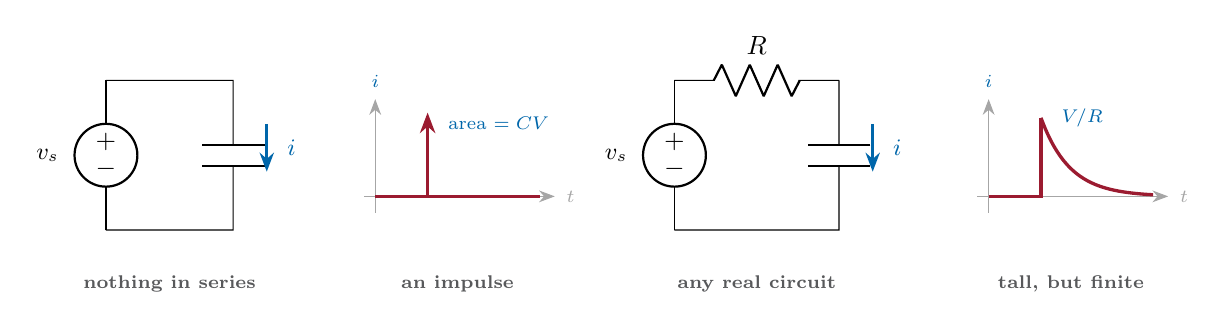
\begin{tikzpicture}[scale=0.95, transform shape]
%---- circuit A : ideal
\begin{scope}
  \draw (0,0) to[american voltage source, invert] (0,2.0);
  \draw (0,2.0) -- (1.7,2.0) to[C] (1.7,0) -- (0,0);
  \draw[iar] (2.15,1.42) -- (2.15,0.78);
  \node[ccur, font=\small] at (2.48,1.1) {$i$};
  \node[font=\small] at (-0.78,1.0) {$v_s$};
  \node[ttl] at (0.85,-0.72) {nothing in series};
\end{scope}
%---- waveform A
\begin{scope}[xshift=3.6cm, yshift=0.45cm]
  \taxes{2.4}{0.22}{1.3}{\Icol{$i$}}
  \draw[crv] (0,0) -- (0.7,0);
  \draw[crv, -{Stealth[length=2.6mm]}] (0.7,0) -- (0.7,1.12);
  \draw[crv] (0.7,0) -- (2.2,0);
  \node[font=\scriptsize, text=ccur, right=2pt] at (0.78,0.98) {area $= CV$};
  \node[ttl] at (1.1,-1.17) {an impulse};
\end{scope}
%---- circuit B : with series R
\begin{scope}[xshift=7.6cm]
  \draw (0,0) to[american voltage source, invert] (0,2.0);
  \draw (0,2.0) to[R, l=$R$] (2.2,2.0);
  \draw (2.2,2.0) to[C] (2.2,0) -- (0,0);
  \draw[iar] (2.65,1.42) -- (2.65,0.78);
  \node[ccur, font=\small] at (2.98,1.1) {$i$};
  \node[font=\small] at (-0.78,1.0) {$v_s$};
  \node[ttl] at (1.1,-0.72) {any real circuit};
\end{scope}
%---- waveform B
\begin{scope}[xshift=11.8cm, yshift=0.45cm]
  \taxes{2.4}{0.22}{1.3}{\Icol{$i$}}
  \draw[crv, domain=0:1.5, samples=90, smooth] plot ({0.7+\x}, {1.05*exp(-2.6*\x)});
  \draw[crv] (0,0) -- (0.7,0) -- (0.7,1.05);
  \node[font=\scriptsize, text=ccur, right=2pt] at (0.78,1.05) {$V/R$};
  \node[ttl] at (1.1,-1.17) {tall, but finite};
\end{scope}
\end{tikzpicture}
\end{center}
\vspace{-2pt}

On the left there is nothing to limit the current. Differentiate the step as in
Section~\ref{sec:impulse}:
\[
  \Icol{i(t)} \;=\; C\,\frac{d\Vcol{v}}{dt} \;=\; C\,V\,\delta(t) ,
\]
an impulse of area $CV$ --- exactly the charge the capacitor must end up holding, delivered
in zero time. The model is telling us that an ideal voltage step across an ideal capacitor
is one idealisation too far.
\vspace{3pt}

On the right the resistance limits the current to $V/R$ at the instant of the step, and
from there it decays while the capacitor voltage rises smoothly to $V$. That is what really
happens, and we will solve this circuit properly when we reach first-order transients.
\end{examplebox}

\begin{examplebox}[Example 4.3 --- reading a current waveform]
The same $1\uni{\mu F}$ capacitor, now fed the current below, starting from
$\Vcol{v(0)} = 0$. Between the corners $\Icol{i}$ is constant, so $\Vcol{v}$ is a straight
line whose slope is $\Icol{i}/C$; where $\Icol{i} = 0$ the voltage simply holds.

\begin{center}
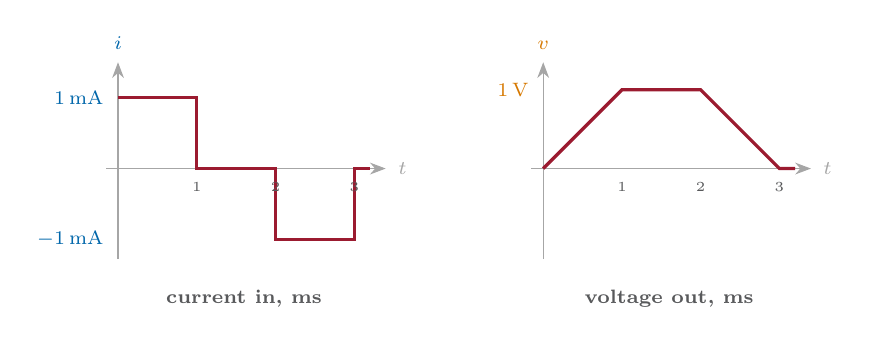
\begin{tikzpicture}[scale=1.0]
\begin{scope}
  \taxes{3.4}{1.15}{1.35}{\Icol{$i$}}
  \draw[crv] (0,0.9) -- (1.0,0.9) -- (1.0,0) -- (2.0,0) -- (2.0,-0.9) -- (3.0,-0.9)
             -- (3.0,0) -- (3.2,0);
  \node[font=\scriptsize, text=ccur, left] at (-0.06,0.9) {$1\uni{mA}$};
  \node[font=\scriptsize, text=ccur, left] at (-0.06,-0.9) {$-1\uni{mA}$};
  \foreach \x/\lb in {1.0/{1}, 2.0/{2}, 3.0/{3}}{
    \node[font=\tiny, text=metugray, below] at (\x,-0.06) {\lb};}
  \node[ttl] at (1.6,-1.65) {current in, ms};
\end{scope}
\begin{scope}[xshift=5.4cm]
  \taxes{3.4}{1.15}{1.35}{\Vcol{$v$}}
  \draw[crv] (0,0) -- (1.0,1.0) -- (2.0,1.0) -- (3.0,0) -- (3.2,0);
  \node[font=\scriptsize, text=cvolt, left] at (-0.06,1.0) {$1\V$};
  \foreach \x/\lb in {1.0/{1}, 2.0/{2}, 3.0/{3}}{
    \node[font=\tiny, text=metugray, below] at (\x,-0.06) {\lb};}
  \node[ttl] at (1.6,-1.65) {voltage out, ms};
\end{scope}
\end{tikzpicture}
\end{center}
\vspace{-2pt}
Up at $1000\uni{V/s}$ for a millisecond, flat for a millisecond, then down again --- and
the capacitor ends where it started, having given back exactly the charge it took. Read
the two pictures the other way round and you have the differentiating view: the voltage's
slope \emph{is} the current, to within the factor $C$.
\end{examplebox}

%==============================================================
\section{Power and energy in an LTI capacitor}
\label{sec:energy}

\[
  \Pcol{p} \;=\; \Vcol{v}\,\Icol{i} \;=\; \Vcol{v}\,C\,\frac{d\Vcol{v}}{dt}
  \;=\; \frac{d}{dt}\!\left(\tfrac12 C \Vcol{v}^{\,2}\right)
  \qquad\Longrightarrow\qquad
  \boxed{\;\Pcol{w} \;=\; \tfrac12 C\,\Vcol{v}^{\,2} \;=\; \frac{\Qcol{q}^{\,2}}{2C}\;}
\]

So the power is the rate of change of $\tfrac12 C \Vcol{v}^{\,2}$. That quantity is the
\textbf{energy the capacitor holds}, and it depends only on the present voltage --- not on
how the capacitor got there.

\begin{center}
\small
\begin{tabular}{@{}l l l@{}}
\toprule
 & \textbf{LTI resistor} \footnotesize(Lecture 3) & \textbf{LTI capacitor}\\
\midrule
terminal equation & $\Vcol{v} = R\Icol{i}$ & $\Icol{i} = C\,d\Vcol{v}/dt$\\
plane it lives in & $\Vcol{v}$--$\Icol{i}$ & $\Vcol{v}$--$\Qcol{q}$\\
memory            & none & the whole past of $\Icol{i}$\\
power $\Pcol{p}$  & $R\Icol{i}^2 \ge 0$ always & $\tfrac{d}{dt}(\tfrac12 C\Vcol{v}^2)$, either sign\\
energy            & dissipated as heat, gone & stored, and all of it returnable\\
verdict           & passive, \emph{lossy} & passive, \emph{lossless}\\
\bottomrule
\end{tabular}
\end{center}

$\Pcol{w} = \tfrac12 C\Vcol{v}^2 \ge 0$, so a capacitor can never give out more than it has
been given: it is passive. But $\Pcol{p}$ goes negative whenever $|\Vcol{v}|$ falls, and
then the capacitor is handing energy back to the circuit. Nothing is lost on the way in or
on the way out.

\begin{ideabox}[For the mechanically minded]
Compare the terminal equation with Newton's second law:
\[
  \Icol{i} = C\,\frac{d\Vcol{v}}{dt}
  \qquad\longleftrightarrow\qquad
  F = m\,\frac{du}{dt} .
\]
Current plays the part of force, voltage the part of velocity, and capacitance the part of
mass --- the same pairing as the mechanical column of Lecture~1. The energies match too:
$\tfrac12 C\Vcol{v}^{\,2}$ against $\tfrac12 m u^2$.\\[3pt]
A heavy flywheel is a large capacitance: a finite force cannot change its speed instantly,
just as a finite current cannot change a capacitor's voltage instantly.
\end{ideabox}

\begin{examplebox}[Example 4.4 --- how much energy is that?]
A $100\uni{\mu F}$ capacitor charged to $12\V$ holds
\[
  \Pcol{w} = \tfrac12 (10^{-4})(12)^2 = 7.2\uni{mJ} .
\]
Enough to light a small LED for a few seconds --- and about what a camera flash unit dumps
into the lamp in a millisecond, which is the point of using a capacitor rather than the
battery directly.
\end{examplebox}

%==============================================================
\section*{Summary}
\addcontentsline{toc}{section}{Summary}

\begin{itemize}
  \item A capacitor is an \textbf{ideal energy-storage element}: it dissipates nothing,
        and everything put in can be taken back out. Every element of Lecture~3 did the
        opposite --- it dissipated all of it.
  \item A \textbf{capacitor} is a curve in the $\Vcol{v}$--$\Qcol{q}$ plane, not the
        $\Vcol{v}$--$\Icol{i}$ plane. It is not a resistor: there is no $f$ with
        $\Icol{i(t)} = f(\Vcol{v(t)})$, because the current follows how $\Vcol{v}$ is
        changing, not what it is.
  \item Parallel plates: $C = \varepsilon A/d$, in farads.
  \item The \textbf{LTI capacitor} has $\Qcol{q} = C\Vcol{v}$, hence
        $\Icol{i} = C\,d\Vcol{v}/dt$ and
        $\Vcol{v(t)} = \Vcol{v(t_0)} + \frac1C\int \Icol{i}\,d\tau$.
        Open circuit at DC; voltage cannot jump; it remembers.
  \item Constant current in gives a voltage \textbf{ramp}; a voltage \textbf{step} would
        demand $\Icol{i} = CV\delta(t)$, an \textbf{impulse} --- the limit of a rectangle
        of height $h$ and width $1/h$, defined by its area and not by any value. That is
        the model's way of saying that some series resistance is always there.
  \item $\Pcol{w} = \tfrac12 C\Vcol{v}^2 = \Qcol{q}^2/2C$: stored, not spent --- and fixed
        by the present voltage, however the capacitor got there. Passive and
        \emph{lossless}, unlike the resistor.
\end{itemize}

\subsection*{Next lecture}
The inductor --- the second ideal energy-storage element, and the mirror image of everything
above: flux linkage and current in place of charge and voltage, $\tfrac12 L\Icol{i}^2$ in
place of $\tfrac12 C\Vcol{v}^2$. With those two elements the course has all it needs to
build circuits that do more than divide.

\subsection*{Reading}
\begin{itemize}
  \item Alexander \& Sadiku, \emph{Fundamentals of Electric Circuits}, Chapters~2 and~6.
  \item Chua, Desoer \& Kuh, \emph{Linear and Nonlinear Circuits}, Chapters~2 and~3.
  \item Lecture notes and videos of Prof.\ Emre Tuna,
        \href{https://users.metu.edu.tr/etuna/ee201/}{\texttt{users.metu.edu.tr/etuna/ee201}}
        --- Lecture~4 video: capacitor $13{:}40$, parallel plates $17{:}24$, LTI
        capacitor $21{:}30$, examples $27{:}40$ and $36{:}19$, power $39{:}31$.
\end{itemize}

\end{document}
